\subsection{Neural network design, training and classification}
\label{sec:des-class}
Two trained networks networks are used to identify the text and writer of each line. Both extract features of the text with the same convolutional architecture, but their trained weights and output heads are separate. A 'head' is the last section of the model which converts the abstract features learnt by the model into the network's final prediction. The text reader using a CNN and BiLSTM sequence model based off of research, implemented from first principles.~\cite[pp.~4--5]{kizilirmak2023}. The writer head combines features across the line, also implemented from first principles. The literacture review explores explanations about the different types of classifiers and the layers within it.

\subsubsection{Training data, labels and evaluation separation}
IAM lines~\cite{marti2002} and photographed samples provide transcripts and writer labels. The evaluated set to train author classification contains six IAM writers (150, 152, 153, 384, 552 and 588) and five personal contributors, to meet R6 of the project proposal which states the system must be able to store minimum 10 author's glyphs and styles at once. The personal pages were written on paper, photographed with the USB camera model setup and paired with line transcripts. The eleven-writer set defines the reported classifier and stored style profiles. The text classifier however was trained off of an extended Teklia IAM dataset with cut crops that are pre-labelled. The author classifier could not use the Teklia IAM dataset due to the fact that it was not labelled with its author.

The writer dataset contains 517 IAM and 669 personal lines. One IAM page per writer is held out, while a seeded 15\% split selects which personal lines are used to validate the training. This gives 1031 training and 155 hold-out lines. The final common evaluation contains 156 re-extracted lines, so it is reported separately from training validation. The text reader uses a joint corpus of Teklia pre-cut IAM and personal lines. 

The main difference between the full page IAM dataset used for author classifier training, and the Teklia full line version of the IAM dataset, is that the full page IAM dataset was split by author, therefore ideal for author training, yet a labelled transcript per page was not available. Manual verification had to be done to ensure the labelling and segmentation was done correctly on the full page IAM dataset. The Teklia IAM set was split by line, and had transcriptions of the cropped line, yet did not have the author who wrote it. This was ideal for the text classifier as the transcriptions did not have to be manually verified to ensure accurate text to label data, and the author was not required since it is used for training the text classifier, which is independent of who wrote it.

Blank or unusable lines and printed prompts are excluded before pairing crops with labels. Augmentation stays within the training partition, to reduce overfitting on lines not trained on. Both the author classifier and the text classifier were verified against their own respective hold out pages, since they were not necessarily the same pages or lines, since the text classifier was trained without knowledge of the author who wrote it, while the author classifier had to.

\subsubsection{Shared convolutional feature extractor}
The input is a batch of grey $64\times640$ line crops, shaped $(B,1,64,640)$ for batch size $B$, as described in the previous section, without stretching the image disproporionately. Intensity scaling to $[-1,1]$ makes dark ink positive and white padding negative. A learned kernel $W$ (the weights) and bias $b$ calculate local responses from input $X$~\cite[pp.~6--8]{lecun1998}. The following equation describes how the a kernal slides across an input tensor ($X$) to compute a local feature map $Z$.
\begin{equation}
z_{o,y,x}=b_o+\sum_c\sum_{i,j}W_{o,c,i,j}X_{c,y+i,x+j}.
\label{eq:des-conv}
\end{equation}
The sums include the input channels and kernel positions. Input patches are rearranged into a matrix for multiplication by flattened kernels, to not have to use standard Python calculation loops for every pixel operation~\cite{chellapilla2006}.

Batch normalisation uses a channel mean $\mu_B$ and variance $\sigma_B^2$ during training, followed by learned coefficient $\gamma$ and offset $\beta$~\cite[pp.~4--5]{ioffe2015}.
\begin{equation}
\widehat z=\frac{z-\mu_B}{\sqrt{\sigma_B^2+\epsilon}},\qquad
y=\gamma\widehat z+\beta.
\label{eq:des-bn}
\end{equation}

The constant $\epsilon$ is used to stabilise division. Inference uses stored running statistics. The activation function, ReLU, applies $\max(0,y)$, used to keep positive responses with a simple nonlinear operation. Max pooling keeps the strongest response from each local window. Table~\ref{tab:des-backbone} describes the features of the architecture.
\begin{table}[!htbp]\centering\small
\begin{tabularx}{\linewidth}{|l|X|l|}
\hline\textbf{Stage}&\textbf{Operation}&\textbf{Output excluding batch}\\\hline
Input&Resized crops to input size and intensity scaling&$1\times64\times640$\\\hline
1&Two $3\times3$ convolutions, each with batch normalisation and ReLU, and $2\times2$ max pool&$32\times32\times320$\\\hline
2&Four convolution/normalisation/ReLU blocks, and $2\times2$ max pool&$64\times16\times160$\\\hline
3&Six convolution/normalisation/ReLU blocks&$128\times16\times160$\\\hline
Height reduction&Maximum over the remaining height&$128\times1\times160$\\\hline
\end{tabularx}
\caption{Convolutional stages and feature dimensions.}
\label{tab:des-backbone}
\end{table}

Two spatial poolings make the width smaller to 160 columns. The final max over height leaves 128 features per column. Figure~\ref{fig:des-firstfeatures} shows the input Owen line and three strong feature channels before the first spatial pool. Their scales are independent, so darkness cannot be compared as an absolute value between channels. The complete layer sequence is retained in Figure~\ref{fig:vt-featurestack} in the appendix.
\begin{figure}[H]\centering
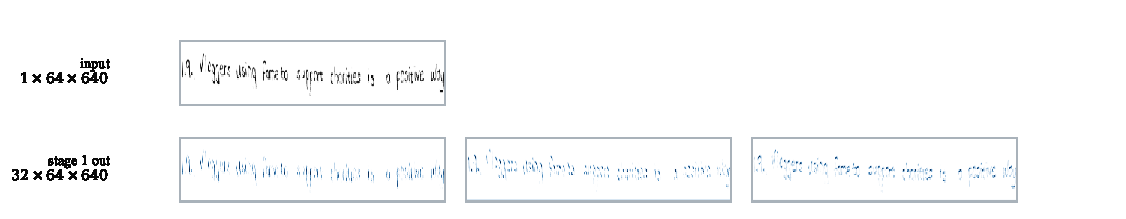
\includegraphics[width=0.90\linewidth]{Figures/design-owen-first-features.pdf}
\caption{Input line and first convolutional features.}
\label{fig:des-firstfeatures}
\end{figure}

\subsubsection{Text recognition using sequence modelling and CTC}
Figure~\ref{fig:des-network} shows the architecture of the text classifier. It consists of two bidirectional LSTM layers, each with 256 hidden units per direction, process the 160 feature columns. The first receives 128 features per frame. The second receives 512 after both directions are concatenated. A linear layer calcultions and determines scores for 74 characters and blank. The writer classifier does not use recurrent layers (the bidirectional LSTM layers are recurrent).
\begin{figure}[H]\centering
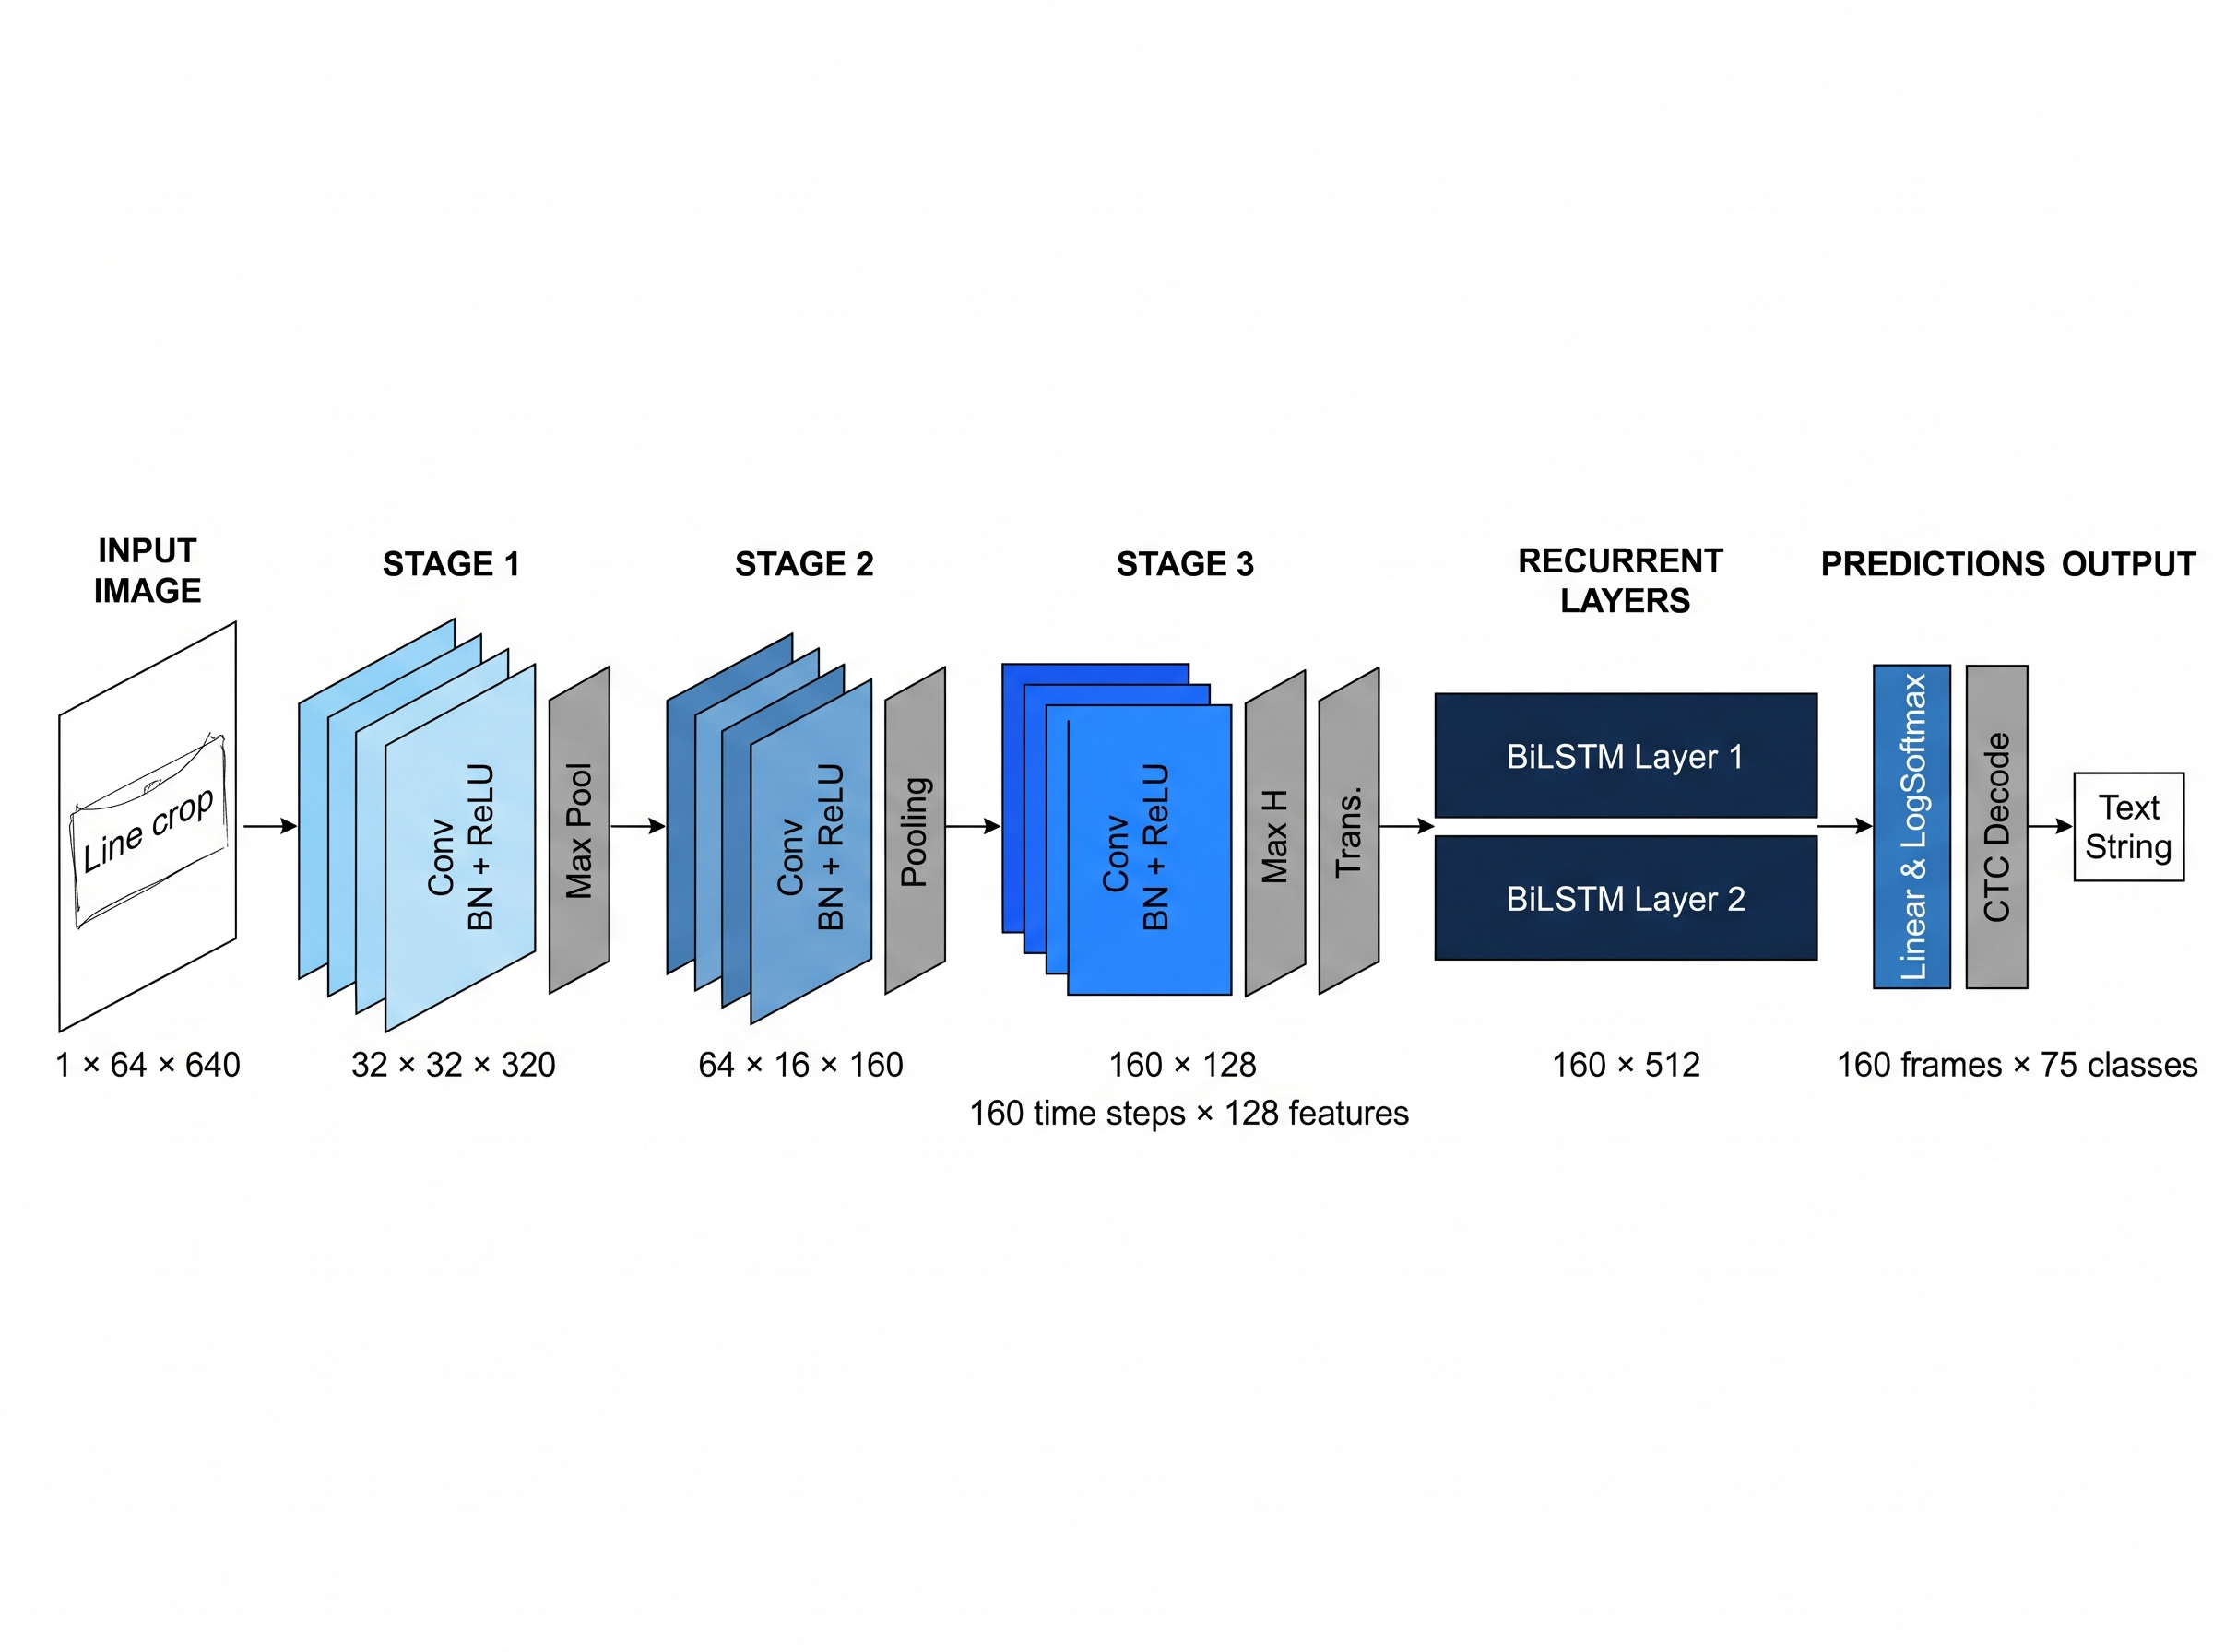
\includegraphics[width=0.96\linewidth,trim=0 130bp 0 134bp,clip]{Figures/BiLSTMCRNN.jpeg}
\caption{Text-reader architecture.}
\label{fig:des-network}
\end{figure}

The LSTM cell state $c_t$ is used to carry and transfer memory and weights between frames. Input, forget and output gates are $i_t,f_t,o_t$, with desired update variable $g_t$ and hidden output $h_t$~\cite[p.~5]{graves2013}.
\begin{equation}
c_t=f_t\odot c_{t-1}+i_t\odot g_t,\qquad
h_t=o_t\odot\tanh(c_t).
\label{eq:des-lstm}
\end{equation}

The gates depend on a vector of the current feature, and the previous hidden state. Sigmoid $\sigma(a)=1/(1+e^{-a})$ is used to limit the gates between zero and one, while $\tanh$ bounds the desired update change. The reverse direction (bidirectional LSTM) supplies context from the other end of the line, to allow the entire line to contribute to the context while classifying. This is particularly useful for cursive words, where all characters in a word are connected and influence the appearance of the word. 

CTC (Connectionist Temporal Classification) is used to train from a line transcript without having the actual labelled character positions~\cite[pp.~2--3]{graves2006}. It gets the total of the frame paths $\pi$ whose collapse $B$ produces a sentence of text $\ell$, using the probabilities $p_t$ over 160 frames.
\begin{equation}
 L_{\mathrm{CTC}}=-\log\sum_{\pi:B(\pi)=\ell}
\prod_{t=1}^{T}p_t(\pi_t).
\label{eq:des-ctc}
\end{equation}

The collapse of the scattered text merges consecutive repeats of characters before removing blanks. Thus a,a,BLANK,b,b becomes ``ab'', while a,BLANK,a gives ``aa''. The dynamic collapse and merging system uses blank-interleaved target states and log probabilities. For $L$ labels and $r$ adjacent repeated pairs, at least $L+r$ frames are required to compute.

A method called 'greedy inference' chooses the most likely class at each frame and then performs the collapse on the text. No language model is ever used to help it. Figure~\ref{fig:vt-lattice} compares greedy decoding with alignment constrained to the known Owen transcript. This line is a worked example containing adjacent \texttt{g}s, which require separated emission runs. The greedy result matches its transcript and blank carries about 46\% of mean frame probability.
\begin{figure}[H]\centering
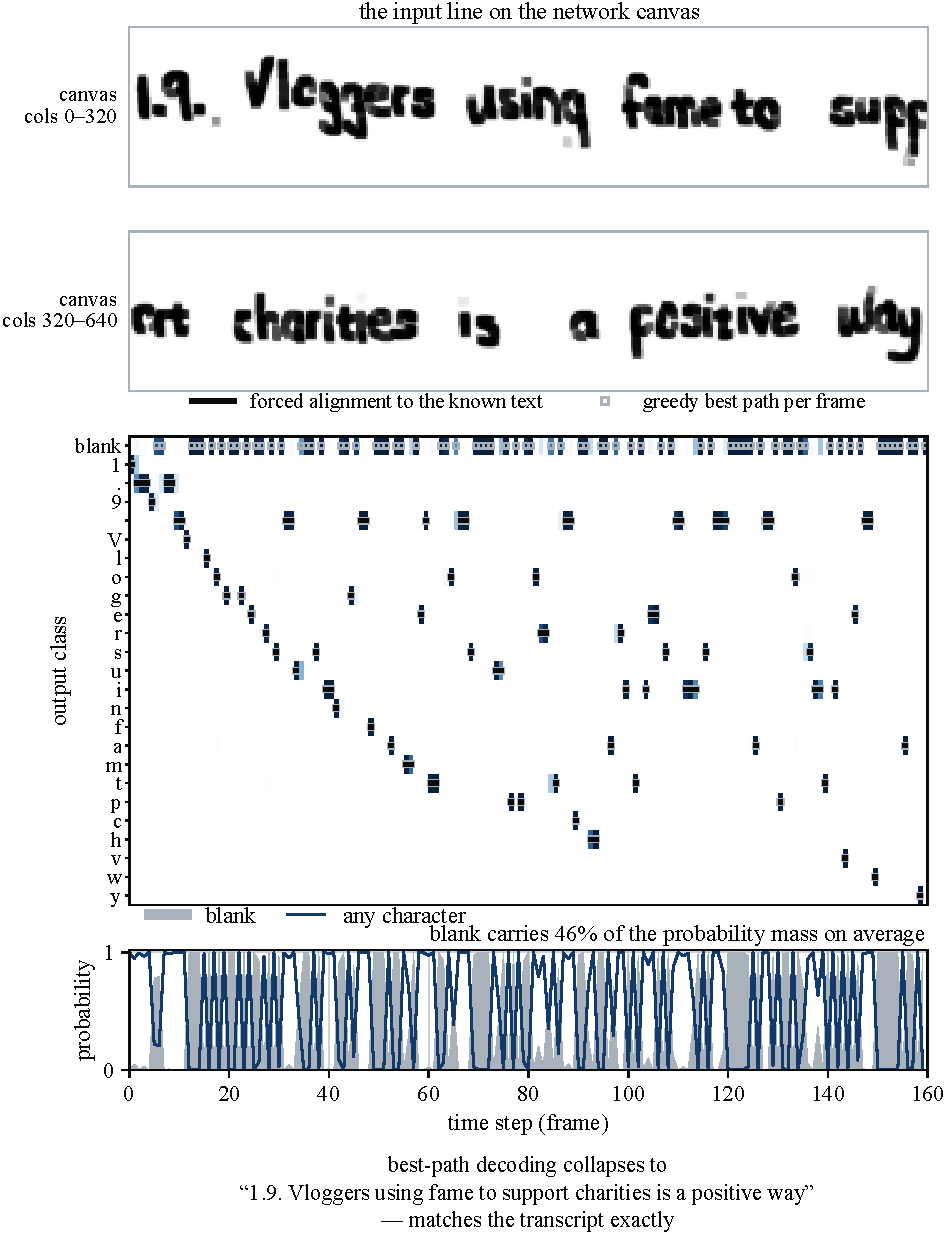
\includegraphics[width=0.96\linewidth]{Figures/VisualTests/T36_ctc_lattice.pdf}
\caption{CTC decoding and forced alignment.}
\label{fig:vt-lattice}
\end{figure}

The numerical backward pass makes use of a target state occupancy $q_{t,k}$ and total path likelihood $Z$ and logits $z_{t,k}$ (which represent the score of the final character guesses). Forward score $\alpha$ includes the current emission (the current network's character guess score) and moves forward though the sequence, while backward score $\beta$ includes only later emissions (future time steps and the prediction at that point) and moves backwards through the sequence~\cite[pp.~4--6]{graves2006}.
\begin{equation}
q_{t,k}=\sum_{s=k}\exp(\alpha_{t,s}+\beta_{t,s}-\log Z),
\qquad \frac{\partial\mathcal L}{\partial z_{t,k}}=p_t(k)-q_{t,k}.
\label{eq:des-ctcgrad}
\end{equation}

The batch average is then applied without target-length division in the trainer, which means that the normalization over target length is skipped and every sequence has equal weight in the calculation regardless of how many characters there are. 

\subsubsection{Writer identification and stroke normalisation}
\label{sec:des-shapenamer}
The writer head averages the 160 feature columns into 128 values and does not use a recurrent layer, because the writers depend directly on the extracted features, and not time units or extended like context. A 96-unit hidden layer, ReLU and a $K$-class output identify the writer. Dropout probability of 0.2 is only used during the training of the network~\cite[pp.~1931, 1934]{srivastava2014}.

The first classifier used the ink styles and thickness from the page scans directly to classify authors. Ink width is a useful writer identifier~\cite[p.~162]{brink2012}, but the gantry uses its own pen, and keeps its ink size consistent, therefore this kind of system is inadequate to be tested with reproduced text. The later classifier therefore uses normalised strokes (with the ink levels standardized for all authors) so that original and reproduced writing are compared more through their geometry. Binarisation, Zhang-Suen thinning and square dilation form are used to form that input, as the following equations describe respectively:~\cite[p.~237]{zhang1984},~\cite[p.~533]{haralick1987}.
\begin{equation}
I_s=255\left[1-\delta_k\bigl(\operatorname{thin}(M)\bigr)\right],\quad
w=\operatorname{clip}\bigl(\operatorname{round}(\rho h_x),2,9\bigr),\quad
k=2\lfloor w/2\rfloor+1.
\label{eq:des-strokenorm}
\end{equation}

where $h_x$ is estimated x-height, $\rho$ is the width fraction and $k$ is the dilation-kernel size. The selected fraction is 0.17, which was obtained from a sweep through various different $\rho$ values to identify the value that produced the best writer identification accuract per page, using the same eleven writers and held-out partition, with a 50-epoch budget for each width. Important caveat here compared to final results, the the results here only did a full page identification test, not a per line test as will be done in the final qualification test, hence the reason the numbers may appear inflated. The important distinquishing factor is the comparison between the four and which is the most accurate. Table~\ref{tab:des-widthselection} gives the best saved epoch and validation score.
\begin{table}[!htbp]\centering\small
\begin{tabular}{|c|c|c|}
\hline\textbf{Width fraction $\rho$}&\textbf{Best saved epoch}&\textbf{Held-out writer accuracy per line}\\\hline
0.06&38&98.06\%\\\hline
0.09&43&97.42\%\\\hline
0.11&39&98.06\%\\\hline
0.17&43&99.35\%\\\hline
\end{tabular}
\caption{Stroke-width selection using the same eleven-writer population and held-out partition.}
\label{tab:des-widthselection}
\end{table}

The best observed width was 0.17. The final author classifier trained from first principles used for results was trained with the 0.17 stroke normalization width value. The sweep is simply considered an experiment to find the width coefficient that performed the best, and is not part of the final qualification tests.


Figure~\ref{fig:des-strokenorm} shows author O and A to illustrate different letter shapes under the same preparation. The original ink is reduced to a centreline before a controlled width is restored. Thresholding or thinning can still damage faint and touching strokes.
\begin{figure}[H]\centering
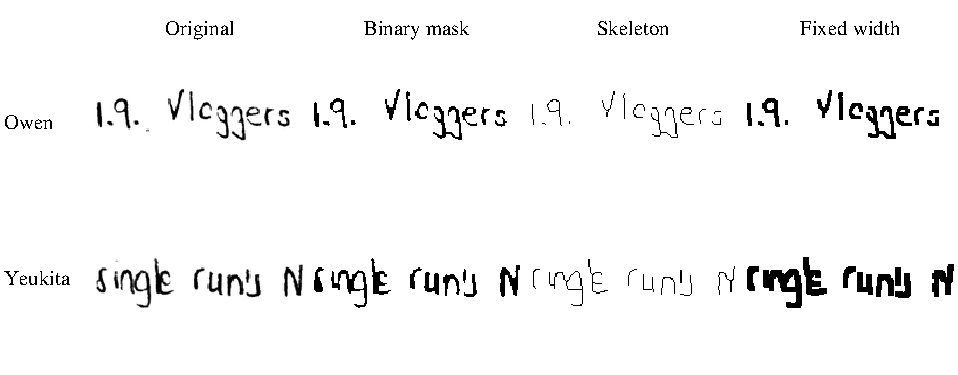
\includegraphics[width=0.98\linewidth]{Figures/design-stroke-normalisation.pdf}
\caption{Stroke normalisation on two writers.}
\label{fig:des-strokenorm}
\end{figure}

\subsubsection{Training procedure and model selection}
\label{sec:des-training}
The backbone and task head are updated together. Training uses convolution weights that are scaled with variance, and initial normalisation scales of one with zero offsets. Augmentation is applied to the training data to create richer model with minimal overfitting, in the form of shear, small rotations, perspective changes and elastic distortion changes to the training images while preserving labels. Validation uses a fixed preparation path without augmentation or dropout.

The text classifier minimises CTC loss, while the author classifier minimises cross-entropy for the true writer $y$, with a logit (score) derivative $p_k-\mathbf1[k=y]$~\cite[p.~6]{graves2013}. Table~\ref{tab:des-training} shows the default rates, optimisers and other methods and coefficients used.
\begin{table}[!htbp]\centering\small
\begin{tabularx}{\linewidth}{|l|X|X|}
\hline\textbf{Setting}&\textbf{Text classifier}&\textbf{Author classifier}\\\hline
Objective&CTC loss&Cross-entropy\\\hline
Optimiser&RMSprop&AdamW\\\hline
Initial learning rate&$10^{-3}$ default&$10^{-3}$ default\\\hline
Weight decay&$10^{-5}$&$10^{-4}$\\\hline
Learning rate changer&Plateau reduction, factor 0.5, patience 5, minimum $10^{-5}$&Cosine annealing over the configured run\\\hline
Gradient norm clipping&Not applied&Maximum norm 5\\\hline
\end{tabularx}
\caption{Training settings implemented in the first-principles trainer. The table describes implemented defaults rather than a recovered record of every completed training run.}
\label{tab:des-training}
\end{table}

The text classifier training supports controlled personal-sample representation, with default fraction 0.20, to ensure there is not biasing between the IAM dataset or personal dataset. Text classifier checkpoints are selected and saved by validation loss and author classifier checkpoints by validation accuracy. Checkpoints were vital to the training, due to the long time it took to train first principles classifiers without libraries or GPU usage capabilities, and a SBC with a mediocre CPU. In case of crashes or power outages, checkpoints were always saved as safety feature, so the run could be continue from the checkpoint. Forward caches kept the quantities needed for differentiation. Algorithm~\ref{alg:des-train} in Appendix~\ref{app:des-training-procedures} gives the update procedure. The supplied first-principles training records are retained in Appendix~\ref{app:training-records}.

\subsubsection{Verifcation through testing with off-the-shelf methods}
\label{sec:des-implementations}
The first principles route implements forward propagation, backward propagation, losses and optimiser updates using NumPy array mathematics. This was verified through a comparison against a PyTorch-implementation of the model. Both used the same image conditioning, data, segmentation, architecture, gradients etc, so they were expected to perform relatively similarly

Table~\ref{tab:dis-training} compares trained models on common original validation material. The text classification scores differ by 0.33 percentage points in favour of the text classifier, and the author classifier differs by 0.57 points in favour of the PyTorch implementation. The PyTorch implementation was expected to perform better than the first principles one, due to the fact that the PyTorch method is optimized, and runs of 64 bit precision floats, while the first principle ones used 32 bit floats to save computation time because they already took many hours to run. A higher precision on float calculations creates more precise error calculations in training. The fact that both methods proved similar results proves the implementation of the model and layer calculations etc. was correct. The difference could be attributed to random augmentation differences between the runs.
\begin{table}[!htbp]\centering\small
\begin{tabularx}{\linewidth}{Xrr}\toprule
\textbf{Common validation material}&\textbf{Library route / \%}&\textbf{First principles / \%}\\\midrule
Reader, public IAM lines&94.12&94.39\\
Reader, photographed lines&93.33&94.42\\
Reader, pooled character accuracy&94.06&94.39\\
Writer, 156 original lines&98.08&97.51\\\bottomrule
\end{tabularx}
\caption{Training-route comparison on common data.}
\label{tab:dis-training}
\end{table}

The error metrics between the PyTorch and first principles versions were recorded aswell, to further prove the consistency between the two implementations to prove the first principles implementation was correct. A numerical comparison was done using identical inputs, parameters and precision, and float64 checks were done between the maximum logit difference (score metrics), the absolute loss difference, and the worst ranked gradient relative difference, show in Table~\ref{tab:des-numericalcheck}. All errors and differences between the two implementations were incredibly small, all less than $10^{-13}$ error margin. Over time these miniscule errors could add up, causing differences in the classifications of each implementation.
\begin{table}[H]\centering\small
\begin{tabularx}{\linewidth}{|X|r|r|}
\hline\textbf{Recorded comparison metric}&\textbf{Reader}&\textbf{Writer classifier}\\\hline
Maximum logit difference / maximum magnitude&$2.12\times10^{-14}$&$3.04\times10^{-15}$\\\hline
Absolute loss difference&$1.14\times10^{-13}$&$1.78\times10^{-15}$\\\hline
Worst ranked gradient relative $L_2$ difference&$2.80\times10^{-13}$&$6.01\times10^{-14}$\\\hline
\end{tabularx}
\caption{Archived float64 operation comparison.}
\label{tab:des-numericalcheck}
\end{table}
